\documentclass[10pt,a4paper,english,italian]{article}
%\usepackage[T1]{fontenc}
\usepackage[latin1]{inputenc}
\usepackage{babel}
\usepackage{amssymb}
\usepackage{amsmath}
\usepackage{epsfig}
\usepackage{tabularx}
\usepackage{multirow}
\usepackage{subfigure}
\usepackage{verbatim}
\usepackage{babel}
\usepackage{fancyhdr}
\usepackage{listings}
\usepackage{psfrag}
\usepackage{color}
\usepackage{../common/espacs}

\makeatother

%\input{../common/commands.tex}

\title{Esercitazione 2}
\date{13/10/2011}
\setlength{\textwidth}{100ex}
\setlength{\oddsidemargin}{0ex}

\pagestyle{fancy}
\headheight 35pt

\begin{document}
\lstset{language=[ISO]C++}
\maketitle

Sia $f\in C^{1}\left(a, b\right)$ una funzione reale che si annulla in
un punto $\alpha\in (a, b)$. Un algoritmo robusto per la
ricerca dello zero di tale funzione pu\`o essere costruito combinando in sequenza l'utilizzo di
un metodo di basso ordine, per cui sia garantita la convergenza globale,
con uno di alto ordine.
Infatti il metodo di alto ordine si avvicina allo zero cercato in un numero inferiore di passi rispetto al metodo di basso ordine, ma pu\`o garantire la convergenza solo partendo da una stima (``guess'') iniziale sufficientemente accurata. Questa stima pu\`o essere fornita tramite qualche passo del metodo di basso ordine, chiamato con una tollerenza larga.


%%%%%%%%%%%%%%%%%%%%%%%

\documentclass[10pt,a4paper,english,italian]{article}
\usepackage[T1]{fontenc}
\usepackage[latin1]{inputenc}
\usepackage{babel}
\usepackage{color}
\usepackage{amssymb}
\usepackage{amsmath}
\usepackage{epsfig}
\usepackage{tabularx}
\usepackage{multirow}
\usepackage{subfigure}
\usepackage{verbatim}
\usepackage{babel}
\usepackage{fancyhdr}
\usepackage{listings}
\usepackage{psfrag}
\usepackage{../common/espacs}

\setlength{\textwidth}{100ex}
\setlength{\oddsidemargin}{0ex}

\pagestyle{fancy}
\headheight 35pt

\rhead{\copyright~Copyright 2007 Daniele A. Di Pietro}

\makeatother

\title{Esercitazione 1}
\author{D. A. Di Pietro}

\setlength{\textwidth}{100ex}
\setlength{\oddsidemargin}{0ex}

\begin{document}
\maketitle
% Set language
\lstset{language=[ISO]C++}

Il calcolo degli autovalori di una matrice \`e richiesto in molte
applicazioni ingegneristiche: un esempio classico \`e l'analisi delle
frequenze naturali di sistemi fisici. I metodi numerici per il calcolo
degli autovettori si distinguono in \emph{parziali}, adatti al calcolo
degli autovalori estremi, e \emph{globali}, in grado di approssimare
l'intero spettro della matrice.

Il \emph{metodo delle potenze} \`e applicabile a matrici in cui
l'autovalore di modulo massimo $\lambda_1$ abbia molteplicit\`a
unitaria e sia ben separato dall'autovalore immediatamente pi\`u
piccolo in modulo. Il generico passo dell'algoritmo \`e riportato di
seguito:
\begin{equation*}
\begin{aligned}
{\bf q}\iter{k} &= \frac{ A{\bf q}\iter{k-1} }{ \norm{ A{\bf q}\iter{k-1}}_2 },\\
{\bf \nu}\iter{k} &= {{\bf q}\iter{k}}^T  A {\bf q}\iter{k},\\
{\bf w}\iter{k} &= \frac{ {\bf w}\iter{k-1}A }{ \norm{ {\bf w}\iter{k-1} A}_2 },
\end{aligned}
\end{equation*}
dove con $\nu\iter{k}$, ${\bf q}\iter{k}$ e ${\bf w}\iter{k}$ si sono
indicate, rispettivamente, le approssimazioni di $\lambda_1$ e degli
autovalori destro e sinistro ${\bf x}_1$ e ${\bf y}_1$ ad esso
associati. Vale la seguente stima, utile per determinare un criterio
d'arresto:
\begin{equation*}
\module{ \lambda_1 - \nu\iter{k} } \approx %
\frac{ \norm{ {\bf r}\iter{k} }_2 }{ \module{ {\bf w}\iter{k}\cdot{\bf q}\iter{k} } },
\end{equation*}
dove ${\bf r}\iter{k} \eqbydef A{\bf q}\iter{k} - \nu\iter{k}{\bf
q}\iter{k}$ \`e il residuo all'iterazione $k$-esima.

Il \emph{metodo di Jacobi} consente di approssimare l'intero spettro
di una matrice simmetrica. L'idea dell'algoritmo \`e quella di
ottenere, a partire da $A$, una matrice quasi diagonale
$A\iter{k}\approx D$ ortogonalmente simile ad $A$ che abbia sulla
diagonale principale le approssimazioni degli autovalori di $A$. La
$k$-esima iterazione richiede di fissare una coppia di indici
$\couple{p\iter{k}}{q\iter{k}}$ e costruire, a partire da
$A\iter{k-1}$, la successiva approssimazione $A\iter{k}$ in modo tale
che
\begin{equation}
a\iter{k}_{pq} = 0.
\label{eq:jacobi:cond}
\end{equation}
Tale approssimazione si calcola mediante una opportuna
\emph{trasformazione di Givens}:
\begin{equation*}
A\iter{k} = G(p\iter{k}, q\iter{k}, \theta\iter{k})^T %
A\iter{k-1} %
G(p\iter{k}, q\iter{k}, \theta\iter{k}),
\end{equation*}
dove l'angolo di rotazione $\theta\iter{k}$ \`e determinato in modo da
soddisfare la condizione \eqref{eq:jacobi:cond}. La matrice di Givens
\`e definita come
\begin{equation*}
\function{G}{i,k,\theta} = I_n - Y,
\end{equation*}
essendo $Y\in\mathbb{R}^{n\times n}$ una matrice nulla eccetto che per
i seguenti valori: $y_{ii} = y_{kk} = 1 - \cos\theta $ e $y_{ik} =
-y_{ki} = -\sin\theta$. Fissata la coppia di indici
$\couple{p\iter{k}}{q\iter{k}}$ relativa alla $k$-esima iterazione,
vale la seguente formula per il calcolo delle funzioni trigonometriche
dell'angolo di rotazione (per brevit\`a di notazione si omette l'apice
quando \`e pari a $k$):
\begin{equation*}
\couple{\cos\theta}{\sin\theta} = %
\begin{cases}
    \couple{1}{0} & \Se{a_{pq}\iter{k-1} = 0}, \\
    \couple{1 / \sqrt{1 + t^2}}{t / \sqrt{1 + t^2}} & \Altrimenti,
\end{cases}
\end{equation*}
dove, posto $\eta \eqbydef \left( a_{qq}\iter{k-1} -
a_{pp}\iter{k-1}\right)/{2a_{pq}\iter{k-1}}$:
\begin{equation*}
t = \begin{cases}
    1 / \left( \eta + \sqrt{1 + \eta^2}\right) & \Se{\eta\ge 0}, \\
    -1 / \left( -\eta + \sqrt{1 + \eta^2}\right) & \Altrimenti.
\end{cases}
\end{equation*}
La coppia di indici $\couple{p\iter{k}}{q\iter{k}}$ pu\`o essere
fissata scorrendo la matrice per riga e scegliendo in sucessione le
entrate nella parte strettamente triangolare superiore (metodo di
Jacobi \emph{ciclico}). Terminata una passata completa (\emph{sweep}),
si ricomincia dalla prima riga. Il metodo si arresta quando la
seguente condizione \`e soddisfatta:
\begin{equation*}
\frac{ \norm{ A\iter{k} - \diag{A\iter{k}} }_F }{ \norm{ A }_F } \le %
\mathtt{tol},
\end{equation*}
avendo indicato con $\norm{\cdot}_F$ la norma di Frobenius. Entrambi i
metodi sono descritti pi\`u dettagliatamente in
\cite[\extref{5}]{Quarteroni.Sacco.ea:2000}.

La codifica dei metodi per il calcolo degli autovalori di una matrice
richiede una libreria per la gestione dell'algebra
lineare. L'implementazione C++ proposta beneficia delle capacit� di
astrazione del linguaggio, che consente, mediante la definizione di
tipi utente ed il sovraccaricamento degli operatori, di utilizzare una
notazione che ricalca quella convenzionale. Come vedremo, bench� tale
soluzione appaia senz'altro elegante, pu� non essere la pi�
efficiente, poich� l'astrazione ha un costo computazionale. Inoltre,
esistono numerose librerie che implementano questi costrutti di base,
il cui utilizzo andrebbe considerato prima di scrivere codice specifico.

Si richiede di
\begin{enumerate}
\item prendendo come modello la soluzione proposta per il metodo di Jacobi ciclico, scrivere una classe che implementi il metodo delle potenze;
\item completare l'implementazione della libreria per l'algebra
lineare, aggiungendo la funzionalit� di prodotto matrice per vettore
(\cpp{operator*} per la classe \cpp{Matrix}) e vettore per matrice (\cpp{operator*} binario);
\item derivare una classe \cpp{Hilbert} dalla classe \cpp{Matrix};
\item \label{validazione} validare il codice utilizzandolo per calcolare gli autovalori
della matrice di Hilbert di dimensione $4$, il cui spettro \`e
riportato sotto fino alla quinta cifra significativa:
\begin{equation*}
\sigma\left( H_4\right) = %
\left\{
    1.5002, 1.6914\e{-1}, 6.7383\e{-3}, 9,6792\e{-5}
\right\}.
\end{equation*}
\item per lo svolgimento del punto \ref{validazione} utilizzare una libreria per l'algebra lineare diversa da quella proposta (ad esempio \cpp{ublas}): modificare (se necessario) il codice.
\end{enumerate}

\newpage

\section*{Soluzione}

La \emph{policy} per il parametro \cpp{template} \cpp{Preconditioner}
\`e la disponibilit\`a di un membro \cpp{solve} in grado di ricevere
un \cpp{Vector} e che restituisca un \cpp{Vector}. Una scelta naturale
\`e quindi la definizione di una classe \cpp{Preconditioner},
\cpp{template} rispetto al tipo del vettore.

Il pi\`u semplice precondizionatore \`e il precondizionatore
\emph{identit\`a}.

\lstset{basicstyle=\scriptsize\sf}
\lstinputlisting[caption=L'interfaccia della classe
\cpp{IdentityPrecond},
linerange={14-43}]{./es/src/solver_policies.hpp}
\lstset{basicstyle=\sf}

Un precondizionatore pi\`u complesso pu\`o essere costruito ricorrendo
a librerie di calcolo per il metodo \cpp{solve}, che fornisce la
soluzione del sistema lineare di precondizionamento. Si propone come
esempio un precondizionatore \emph{diagonale}, ottimale per matrice
simmetrica definita positiva \cite{Quarteroni.Sacco.ea:2000}: il solutore utilizzato \`e fornito dalla
libreria \cpp{boost} per sistemi triangolari.

\lstset{basicstyle=\scriptsize\sf}
\lstinputlisting[caption=L'interfaccia della classe
\cpp{UblasTriPrecond},
linerange={45-88}]{./es/src/solver_policies.hpp}
\lstset{basicstyle=\sf}

Si noti il parametro \cpp{template} \cpp{C} per la classe
\cpp{UblasTriPrecond}, posto per \emph{default} uguale a
\cpp{UBLAS::lower_tag}: si tratta di un parametro richiesto dal solver
\cpp{UBLAS::solve} per distinguere una matrice triangolare superiore
da una matrice triangolare inferiore (si veda \cite{UBLASweb}).

Il \emph{main program} \`e riportato di seguito. La lettura delle
matrici da file viene effettuata sfruttando i metodi disponibili per
la classe \cpp{string} della STL. Il sistema lineare \`e risolto con i
due diversi precondizionatori.

\lstset{basicstyle=\scriptsize\sf}
\lstinputlisting[caption=Il \emph{main program}]{./es/main.cpp}
\lstset{basicstyle=\sf}

Il risultato dell'esecuzione \`e il seguente:
\begin{verbatim}
Identity Preconditioner
        status = 0
        number of iterations = 10
        error = 2.78721e-19

Triangular Preconditioner
        status = 0
        number of iterations = 10
        error = 2.78721e-19
\end{verbatim}

Si noti che in questo esercizio l'effetto del precondizionatore diagonale non \`e decisivo
rispetto al caso di matrice non precondizionata (d'altra parte per il
caso in esame il precondizionatore diagonale \`e esattamente un
multiplo della matrice identit\`a).

Le \emph{performances} del codice possono essere
misurate con gli strumenti di analisi \emph{valgrind} e
\emph{gprof}. In particolare \`e interessante valutare l'occupazione di
memoria durante l'esecuzione del programma, in funzione del tipo di
strutture dati.
\begin{verbatim}
valgrind --tool=massif ./main
\end{verbatim}

\begin{figure}
\subfigure[Matrice piena]{
\centering
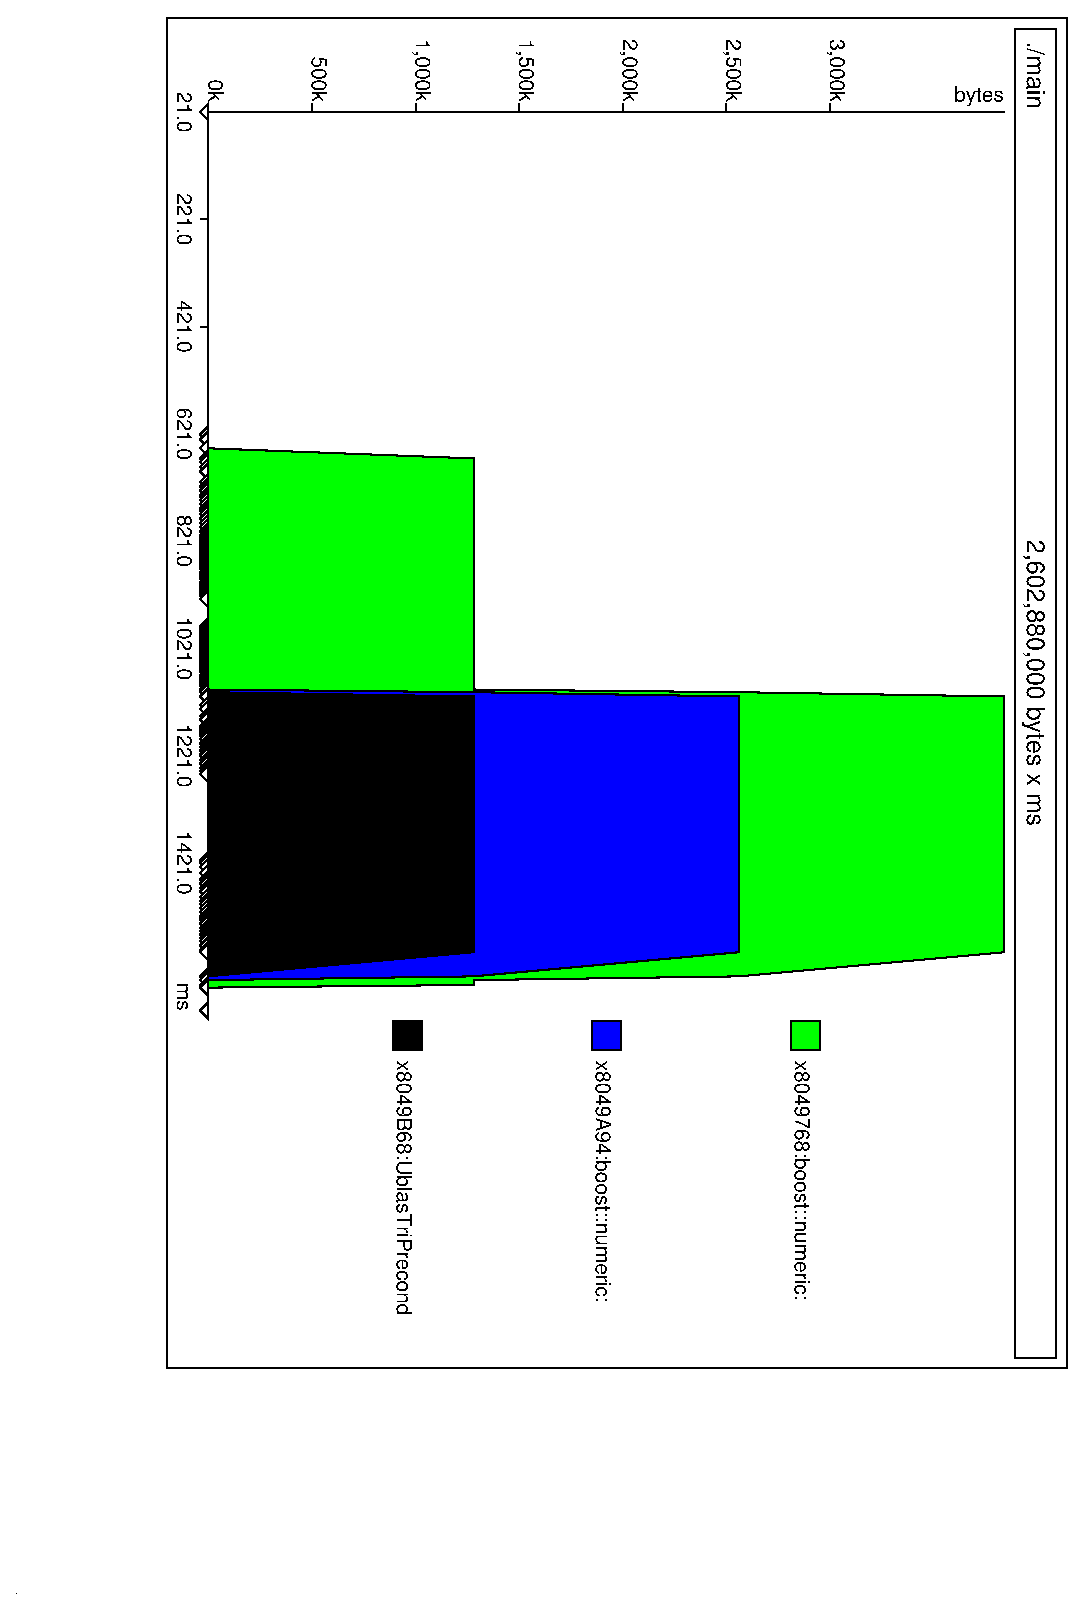
\includegraphics[height=.75\textwidth,angle=-270]{./massif.densebig.eps}
}
\subfigure[Matrice sparsa]{
\centering
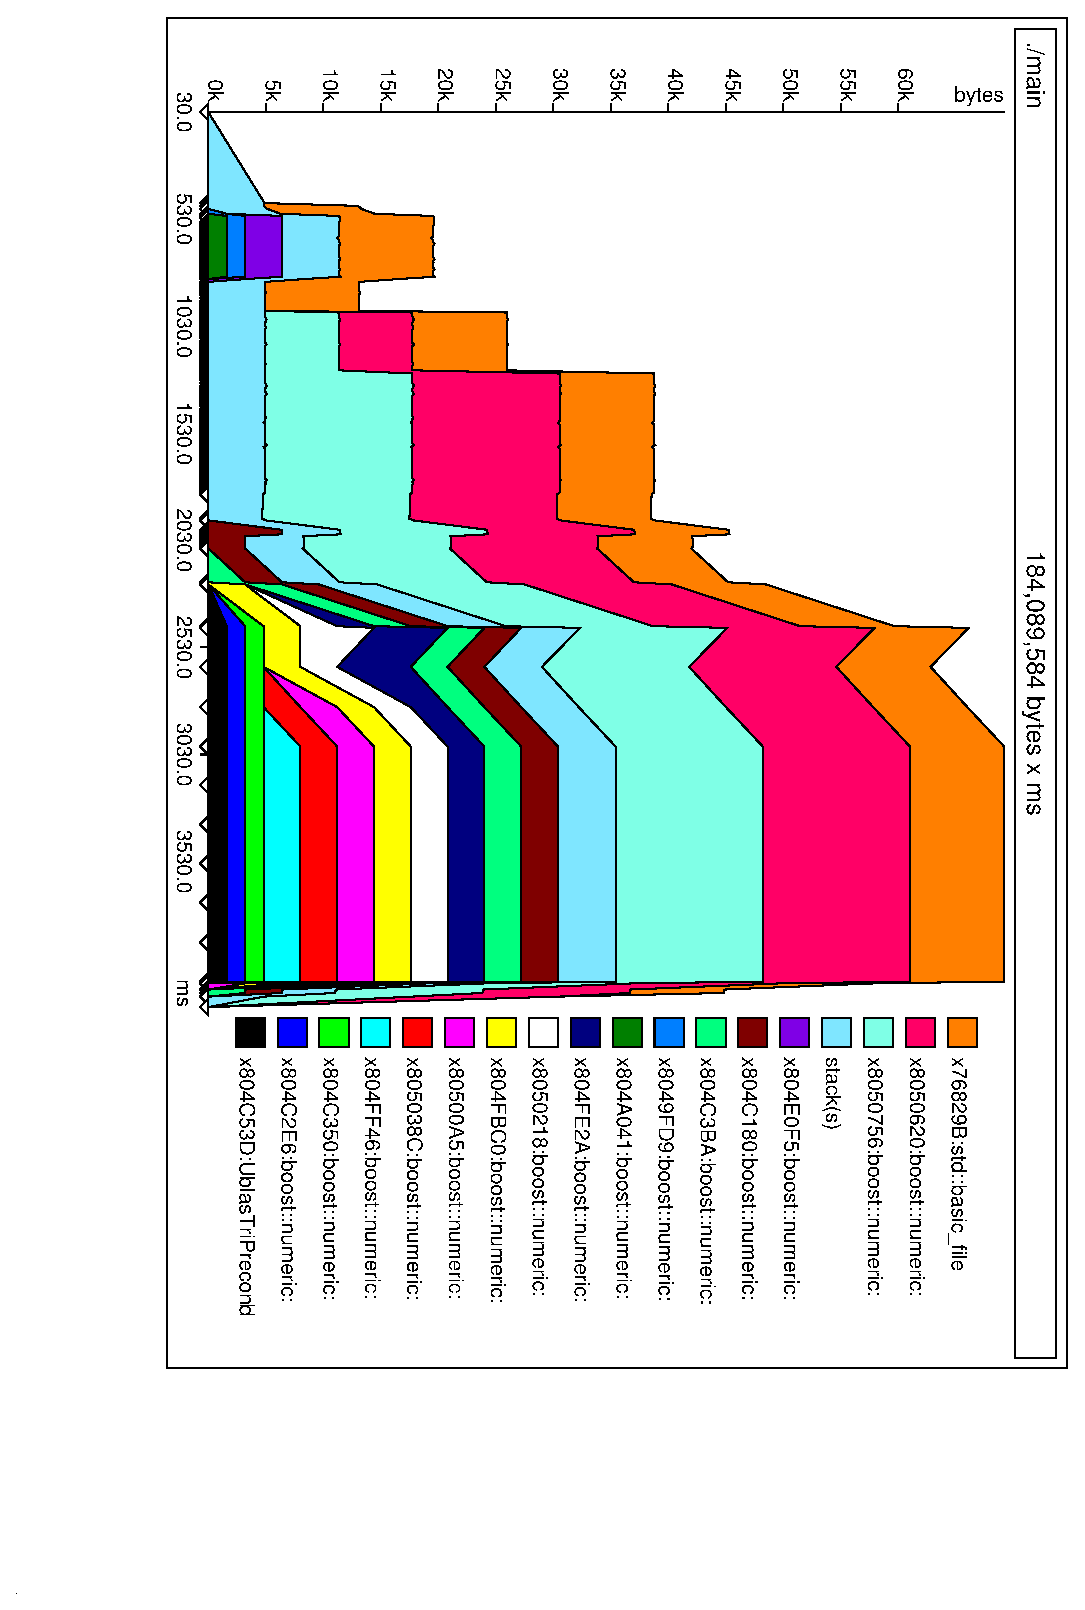
\includegraphics[height=.75\textwidth,angle=-270]{./massif.sparsebig.eps}
}
\caption{Occupazione di memoria durante l'esecuzione del programma,
  per la risoluzione di un sitema lineare quadrato di ordine 400.}
\label{fig:fin:results}
\end{figure}

I grafici generati da \texttt{valgrind} attraverso lo strumento
\texttt{massif} indicano dei valori di occupazione della memoria in
termini di \emph{spazio-tempo}: l'area sottesa alle curve misura
quanta memoria \emph{heap} \`e stata occupata, per quanto tempo. In effetti
il tempo di esecuzione del programma viene influenzato dalle
operazioni svolte da \texttt{valgrind}, quindi il dato pi\`u rilevante
\`e quello ``spaziale'' (in ordinata). In ciascun grafico si nota
quali operazioni del programma ne influenzino maggiormente le
prestazioni; confrontando i due grafici si ha un idea dell'effetto
dell'utilizzo dei due diversi formati di memorizzazione dei
dati. Informazioni dettagliate sulle misure realizzate da
\texttt{valgrind} sono riportate nel file di testo generato come
output. Per ottenere il maggior numero di indicazioni occorre
compilare il \emph{main program} con opzioni di \emph{debug}.

Si noti che, nell'implementazione proposta,
vengono utilizzati i tipi della libreria
\cpp{boost}: quando si utilizzano oggetti di tipo \cpp{matrix}, che
adottano il formato di memorizzazione pieno, l'occupazione della
memoria \`e decisamente pi\`u ingente. Il formato di memorizzazione sparso \`e adottato da
oggetti di tipo \cpp{coordinate_matrix}, grazie ai quali l'occupazione complessiva
di memoria \`e ridotta circa di un fattore 50 (nel caso di matrice
$400 \times 400$).




% Commentare le linee seguenti qualora non vi fossero riferimenti bibliografici
%\bibliographystyle{siam}
%\bibliography{../common/bibliography}

\end{document}

\subsection*{Soluzione}

Viene fornita di seguito un'implementazione del metodo delle potenze
che sfrutta i vettori e le matrici fornite da Eigen.

La classe \cpp{LinearAlgebra::Eigenvalues::Power} possiede un unico
costruttore cui viene passata la tolleranza ed il massimo numero di
iterazioni. La ragione per cui si impone un limite al numero di
iterazioni \`e evitare che, in caso di mancata convergenza, il sistema
entri in un ciclo infinito. Il metodo viene applicato tramite una
chiamata al membro \cpp{apply}, cui va passata la matrice di cui si
vuole calcolare l'autovalore di modulo massimo ed una stima iniziale
dell'autovettore destro ad esso associato. All'intero del codice, viene
utilizzata tale approssimazione anche per inizializzare il calcolo
dell'autovettore sinistro. Il codice relativo alla classe \cpp{Power}
\`e riportato di seguito.
%
\lstset{basicstyle=\scriptsize\sf}
    \lstinputlisting[caption=Interfaccia della classe
        \cpp{Power}]{./es/pagerank-eigen/src/power.hpp}
\lstset{basicstyle=\sf}

Si noti i due \cpp{typedef} definiti pubblici all'inizio della classe.
Tale definizione \`e molto utile, dato che dall'esterno posso utilizzare
tali \cpp{typedef}. Cambiando la definizione all'interno della classe
cambiano automaticamente in tutto il codice. \`E interessante confrontare
la diverse implementazione dei due metodi \cpp{tol()}, oppure \cpp{maxit()}.
La firma di tali metodi differisce unicamente ``dall'ultimo \cpp{const}'' e,
ovviamente, non dal valore di ritorno. Nel primo caso posso modificare esternamente
il valore di \cpp{M_tol}, oppure \cpp{M_maxit}, mentre nel secondo caso no.
\`E stato definito anche il costruttore di copia e l'operatore di assegnazione
come privati, in questo modo inibiamo la possibilit\`a di utilizzarle quelli
di default. L'implementazione di tali metodi \`e inutile.

\lstset{basicstyle=\scriptsize\sf}
    \lstinputlisting[caption=Implementazione della classe
        \cpp{Power}]{./es/pagerank-eigen/src/power.cpp}
\lstset{basicstyle=\sf}

All'inizio del metodo \cpp{apply()} \`e interessante notare l'utilizzo di due tipi
di costruttori per i vettori delle Eigen. Nel primo e nel terzo caso viene utilizzato
il costruttore di copia, mentre nel secondo e quarto caso viene utilizzato il costruttore
che genera il vettore vuoto lungo \cpp{N}.

Il listato contenente il \cpp{main} \`e riportato qui di seguito
\lstset{basicstyle=\scriptsize\sf}
    \lstinputlisting[caption=Interfaccia della classe
        \cpp{Power}]{./es/pagerank-eigen/eig.cpp}
\lstset{basicstyle=\sf}

Notiamo l'utilizzo dei \cpp{typedef} che `` derivano '' dalla classe \cpp{PowerMethod},
tali \cpp{typedef} vengono visti dall'esterno come se la classe \cpp{PowerMethod} fosse
un \cpp{namespace}. Infatti \`e possibile accedere a tali elementi senza creare alcun
oggetto di classe \cpp{PowerMethod}. Tali \cpp{typedef} sono associati alla classe e non
alla particolare istanziazione della stessa.


%%%%%%%%%%%%%%%%%%%%%%

\section*{Esercizio 2 - Da svolgere a casa}

In accordo con l'algoritmo per la generazione di mesh non
equi-spaziate descritto in \textit{A. Quarteroni, Modellistica
Numerica per Problemi Differenziali, 4$^a$ edizione} pagina 398,
in basso. Modificare la classe \cpp{Mesh1D} in modo che possa
creare mesh non equi-spaziate partendo da una funzione peso assegnata.

\subsection*{Soluzione es. 2}

Si riporta di seguito il listato dell'\emph{header file} che contiene
le dichiarazioni delle procedure che risolvono l'esercizio.
% zerofun.hpp
\lstset{basicstyle=\scriptsize\sf}
    \lstinputlisting[caption=Procedure per la ricerca
        degli zeri di una funzione.]{es/1/zerofun.hpp}
\lstset{basicstyle=\sf}

Le corrispondenti definizioni sono state inserite nel \emph{source file}
\texttt{zerofun.cpp}:
\lstset{basicstyle=\scriptsize\sf}
    \lstinputlisting[caption=Procedure per la ricerca degli zeri di una
        funzione.]{es/1/zerofun.cpp}
\lstset{basicstyle=\sf}

L'istruzione \texttt{assert(u*f(b)<0.0);} permette un semplice controllo degli errori,
perch\`e provoca l'interruzione del programma e la generazione di un
messaggio di errore se l'espressione \texttt{u*f(b)<0.0} non \`e verificata.

Infine riportiamo il listato contenente il main nel file \texttt{bn.cpp}:
\lstset{basicstyle=\scriptsize\sf}
    \lstinputlisting[caption=Definizione della funzione e main del programma.]
    {es/1/bn.cpp}
\lstset{basicstyle=\sf}

Per la compilazione si ricorre ai seguenti comandi:
\begin{verbatim}
g++  -c -o bn.o bn.cpp -Wall
g++  -c -o zerofun.o zerofun.cpp -Wall
g++  -o bn bn.o zerofun.o
\end{verbatim}

I \emph{files} \texttt{bn.o} e \texttt{zerofun.o} sono la
rappresentazione in codice oggetto delle definizioni di tipi e
funzioni contenute nei \emph{files} sorgente
(rispettivamente \texttt{bn.cpp} e \texttt{zerofun.cpp}.
Il collegamento (\emph{linking}) dei \emph{files} oggetto
produce l'eseguibile \texttt{bn}.
Per disattivare tutti gli \cpp{assert} all'interno del codice,
in fase di compilazione occorre aggiungere il parametro \cpp{-DNDEBUG}
per quei files che utilizzano gli \cpp{assert}, ovvero
\begin{verbatim}
g++  -c -o bn.o bn.cpp -Wall
g++  -c -o zerofun.o zerofun.cpp -Wall -DNDEBUG
g++  -o bn bn.o zerofun.o
\end{verbatim}

Per visualizzare graficamente l'errore commesso, \`e possibile
aggiungere due parametri di input alle funzioni \texttt{bisection},
\texttt{newton} e \texttt{robust}.
Il primo \`e la soluzione esatta mentre il secondo \`e il nome del
file su cui salvare i dati.
Il listato dei comandi contenuti in \texttt{bng.cpp} \`e il seguente:
\lstset{basicstyle=\scriptsize\sf}
    \lstinputlisting[caption=Definizione della funzione e main del programma.]
        {es/1/withGnuplot/bng.cpp}
\lstset{basicstyle=\sf}

Si noti il comando finale di chiamata al sistema operativo,
\`e richiesto quindi il file \texttt{print\_data} che contiene i seguenti comandi
\begin{verbatim}
set terminal png
set output "grafico.png"
plot "data" with lines
\end{verbatim}
I comandi in \texttt{zerofung.hpp} sono sostanzialmente identici a quelli
riportati in \texttt{zerofun.hpp}, mentre i comandi in \texttt{zerofung.cpp}
sono riportati qui di sequito
\lstset{basicstyle=\scriptsize\sf}
    \lstinputlisting[caption=Procedure per la ricerca degli zeri di una
        funzione.]{es/1/withGnuplot/zerofung.cpp}
\lstset{basicstyle=\sf}

Si noti nella funzione \texttt{bisection} e \texttt{newton} la gestione del file.
Anzitutto viene dichiarato, dove \`e necessario l'operatore di scope resolution
\texttt{::} per accedere ai membri definiti nel namespace \texttt{std}.
Successivamente viene aperto in modalit\`a out nel caso della funzione
\texttt{bisection}, mentre in modalit\`a out e app nella funzione \texttt{newton}.
La differenza \`e che nel secondo caso i dati vengono scritti dal fondo del file.
Vi \`e poi un test per verificare se il file \`e stato effettivamente aperto.
All'interno di cicli vi \`e la scrittura dei dati, i comandi sono analoghi a
quelli utilizzati per la visualizzazione a schermo.
Alla fine di entrambe le funzioni il file viene chiuso.

Il grafico ottenuto \`e il seguente
\begin{figure}[!h]
    \centering
    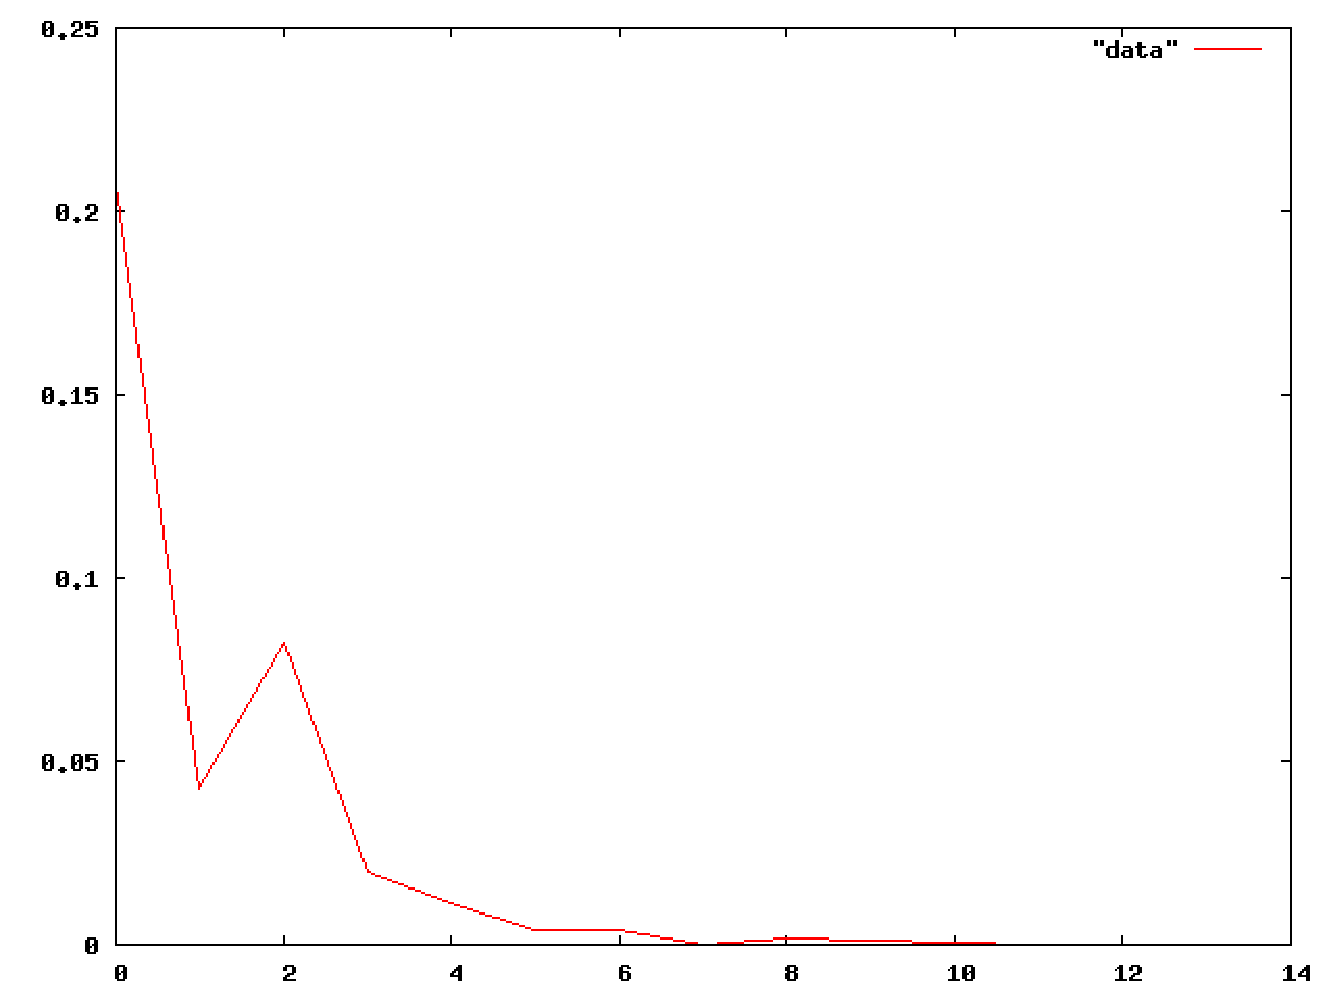
\includegraphics[width=0.7\textwidth]{./images/grafico}
\end{figure}


%%%%%%%%%%%%%%%%%%%%%

\subsection*{Note sui cicli}

Il codice proposto al \emph{Punto 1} utilizza un ciclo \cpp{while}.
%Un' altra alternativa possibile \`e l'uso di un ciclo \texttt{while}:
%\lstset{basicstyle=\scriptsize\sf}
%\lstinputlisting[caption=Ciclo \texttt{while} senza
%\texttt{break}.,linerange={26-47}]{es/1/zerofun-while.cc}
%\lstset{basicstyle=\sf}
In queso caso la prima valutazione della funzione \`e necessariamente esterna
al ciclo.

In alternativa si potrebbe scrivere un ciclo \cpp{for} ed utilizzare
l'istruzione \texttt{break} qualora venisse raggiunta la convergenza entro
il massimo numero di iterazioni.
\lstset{basicstyle=\scriptsize\sf}
    \lstinputlisting[caption=Ciclo \texttt{for} con
        \texttt{break}.,linerange={26-67}]{es/1/old_file/zerofun-break.cc}
\lstset{basicstyle=\sf}
L'istruzione \texttt{break} \`e un modo efficiente per
imporre una condizione di uscita, ma pu\`o rendere il codice di difficile
lettura ed interpretazione; infatti le condizioni di uscita sono sparse e non
sono raggruppate all'inizio o alla fine. Per questo motivo si cerca di limitare
l'uso di \texttt{break} alla gestione di eccezioni.

Una soluzione alternativa \`e basata sul ciclo \cpp{do}/\cpp{while}:
\lstset{basicstyle=\scriptsize\sf}
\lstinputlisting[caption=Ciclo \texttt{do\ldots while} senza
    \texttt{break}.,linerange={26-47}]{es/1/old_file/zerofun-dowhile.cc}
\lstset{basicstyle=\sf}
In questo caso le condizioni di uscita sono chiaramente visibili in fondo al
codice. Il prezzo da pagare \`e un inutile assegnamento di variabili
nell'ultima iterazione eseguita. Il costrutto \texttt{do \ldots while} ha come
caratteristica fondamentale quella di eseguire sempre almeno una iterazione,
anche se le condizioni di uscita non sono verificate o
verificabili all'inzio del ciclo.
A volte questo comportamento pu\`o aiutare a generare errori non banali,
se il codice scritto \`e complesso.



\bibliographystyle{siam}
\bibliography{../common/bibliography}

\end{document}
